% Chapter 1

\chapter{The $R$-matrix method} % Main chapter title

\label{cha:rmatrix} % For referencing the chapter elsewhere, use \ref{Chapter1} 

\lhead{Chapter 3. \emph{The $R$-matrix method}} % This is for the header on each page - perhaps a shortened title

%----------------------------------------------------------------------------------------

\section{Photon and electron interactions}\label{sec:cross}
In this Chapter we will focus first on covering the basic concepts behind the atomic processes of photoionization and electron-impact excitation. We will extend these basic and informal definitions and incorporate them into the $R$-matrix method which follows in the next Section.

We consider some atomic system denoted by $X_i^{q+}$, which is in some initial state $i$. This system can then absorb a photon with enough energy to ionize $X_i^{q+}$ to leave it in the ground state or some excited state, $X_f^{(q+1)+}$ with the ejection of an electron into the continuum. This photoionization process can now be written in the following way,
\begin{equation}\label{eq:rmat_basicphoto}
\begin{split}
& ~~~~~~~~~~~~~~ \tiny{\circled{1}}\\
& h\nu+ X_i^{q+} \rightarrow X_f^{(q+1)+} +e^-\\
& ~~~\tiny{\circled{2}}\searrow ~~~~~~~~~~~~~~~~~\nearrow \tiny{\circled{2}} \\
& ~~~~~~~~~~~~(X_y^{q+})^*
\end{split}
\end{equation}
where $X_i^{q+}$ has some eigenenergy $E_i$, in its initial state with corresponding eigenstate $\Psi_i$. Likewise, $X_f^{(q+1)+}$ is left in some final state with corresponding eigenenergy $E_f$. Finally, the electron that is ejected from the system, otherwise known as a photoelectron, leaves with some momentum $\boldsymbol{k}_f$. The process along the top arrow 1) in equation (\ref{eq:rmat_basicphoto}) is known as direct photoionization. However, following the secondary route 2), we can temporarily excite $X_i^{q+}$ into some autoionization state $y$ before the ejection of the electron. We must also adhere to the conservation of energy, so we can then write the following equation,
\[
h\nu+E_i=\frac{1}{2}k_f^2+E_f.
\]
where we have set the mass of the electron $m_e=1$.

The next important process that we will be covering in this thesis is known as electron-impact excitation and it can also be written informally as,
\begin{equation}\label{eq:rmat_basicelectron}
\begin{split}
& ~~~~~~~~~~~~~~ \tiny{\circled{1}}\\
& e^- + X_i^{q+} \rightarrow X_f^{q+} + e^-.\\
& ~~~\tiny{\circled{2}}\searrow ~~~~~~~~~~~~~~\nearrow \tiny{\circled{2}} \\
& ~~~~~~~~~(X_y^{(q-1)+})^*
\end{split}
\end{equation}
The electron can therefore transfer its energy to make some transition from a lower ($i$) to higher ($f$) energy state as described before for the photoionization process, and is similarly referred to as its 1) direct excitation pathway. Likewise, the electron can become temporarily bound in a resonant state and this is known as the 2) indirect pathway.


\section{$R$-matrix theory}\label{sec:rmatrix}
Despite the non-relativistic $R$-matrix method being implemented first to describe nuclear interactions \citep{1947PhRv...72...29W}, and furthermore generalized to a relativistic approach by \citet{1948PhRv...73.1463G}, it has since been applied to atomic processes based on the fundamental concepts from scattering theory. Due to the substantial complexity of the computer codes, its capabilities are ever changing and improving. To begin this Chapter, we note some of the major advancements in the field that has allowed us to perform such sophisticated calculations. 

It had become clear that these interactions could be understood by the $R$-matrix method by \citet{1968AdAMP...4..173B}. The theory was then first implemented to consider electron-atom collisions \citep{1971JPhB....4..153B}, and resulted in the first $R$-matrix codes in $LS\pi$ coupling \cite{1974CoPhC...8..149B}. The theory of photoionization was then described in the $R$-matrix framework by \citet{1975JPhB....8.2620B}. Further modifications based on the Breit-Pauli Hamiltonian operators are detailed by \citet{1980JPhB...13.4299S}, resulting in the extension to the {\sc bp} suite of codes \citep{1982CoPhC..25..347S, 2001JPhB...34.4455M}. Many of the routines were based on the computer package {\sc civ3} when treating the target state problem, due to its similarities. A general overview can be obtained in the book of \citet{2011rmta.book.....B} and technical documents describing the important routines and variables are presented by \citet{1995CoPhC..92..290B}. However, this is not the extent of its capabilities, further extensions for calculating polarizabilities \citep{1973JPhB....6..945R}, and to include molecular systems \citep{1977JPhB...10.2497B} have also been considered.

The {\sc darc} suite of relativistic codes were based originally on {\sc grasp} \citep{1979CoPhC..17..149G}, and provides an alternative procedure for heavier systems. The theory has been considered by \citet{1975JPhB....8.2327C} and solutions for the asymptotic equations can be obtained by \citet{1994CoPhC..83..215Y}.

This is not the end of the story for $R$-matrix theory, and the above are just a handful of publications amongst many others. These underlying techniques have been implemented to consider a range of other approaches such as the B-splines (code - {\sc bsr}) method by \citet{2006CoPhC.174..273Z} which employs a non-orthogonal basis, or the intermediate-coupling frame transformation method (code - {\sc icft}) by \citet{1998JPhB...31.3713G}, which we will not detail in this thesis.

The $R$-matrix method therefore serves as an ideal set of powerful tools in order to produce accurate atomic observables for a multitude of processes and interactions. With the advancements in technology, larger calculations are now possible and some of the biggest are currently being carried out to date. We will focus now as our main objective to implement $R$-matrix theory so that we can obtain electron-impact excitation and photoionization cross-sections.

We have already defined an informal definition that describes the photon and electron process in equations (\ref{eq:rmat_basicphoto}) and (\ref{eq:rmat_basicelectron}) respectively. In this current Chapter and throughout the thesis, it is wise to adopt the following notation; $X_i^{q+}$ is generally described as the $(N+1)$-electron system, and the residual ion, $X_f^{(q+1)+}$ is regarded as the target ion consisting of $N$-electrons. The system under scrutiny, $X$, is obviously of great importance, and also the initial state $i$ and final residual ion state $f$ will also need to be considered.

In order to apply the $R$-matrix method, we must be able to describe how the ejected continuum electron interacts with the target. The first stage of the theory states that configuration space in spherical polar coordinates is divided into two separate regions, namely an internal region and an external region. This separation can be visualized in Figure \ref{fig:rmat_sphere} for a system with an $N$-electron target, which is represented by the grey colour, and the remaining region past the dashed line is the external region. However, we need some description of the target in order to define an appropriate division of this configuration space. The $R$-matrix boundary radius is determined to be the range of the target, or specifically the radial extent of the most diffuse orbital included.

Two scenarios unveil themselves, the first is when an electron is within the internal region and is therefore considered to be strongly coupled to the target. This is a difficult many-bodied problem to solve as we must describe the various interactions that take place between it and the remaining electrons of the system. The external region describes the $(N+1)^{\rm th}$ ejected electron as being distinguishable and is treated separately as it moves in the long-range Coulomb potential due to the target distribution.

\begin{figure}[hbt]
\centering
\includegraphics[scale=0.55]{Figures/r-matrix/int-ext.pdf}
\caption{The $R$-matrix delineation of internal and external regions in spherical coordinates. Scenario 1 is when the electron is within the internal region, and scenario 2 is when the electron resides in the external region. \label{fig:rmat_sphere}}
\end{figure}

An accurate description of the target is always necessary in these calculations. A truncation of both the target states and the continuum electron is also required in order to provide a tractable problem to solve. We must also consider specifying the coupling scheme required for each calculation. Generally, for heavy atoms/ions then relativistic effects do play a very significant role and some intermediate coupling scheme is adopted, and in this thesis we detail both $jj$ and $jK$. If this is not the case then the target states are described in terms of $LS\pi$ coupling. One result of including relativistic effects, namely the spin-orbit operator in equation (\ref{eq:many_bp3}) is the splitting of the target state terms into fine-structure levels. So not only is additional time required to transform between coupling schemes, but these target state expansions become larger and larger.

We describe the theory of this Section by looking at a non-relativistic $R$-matrix calculation for simplicity, and then consider important extensions, and also the Dirac approach to accurately incorporate additional relativistic effects. The remaining Sections focus on matching the wavefunction at the $R$-matrix boundary and through asymptotic solutions in order to calculated corresponding scattering cross-sections. Finally, an overview of the important routines of each stage of the calculation are considered.

\section{Describing the target}\label{sec:target}
We now need to obtain descriptions for various wavefunction states by its characteristics in the internal and external regions. This is the first step to overcome in $R$-matrix theory, and also provides an appropriate boundary radius r$_a$, for the division of configuration space. Once this has been dealt with, we can then consider the full $(N+1)$-electron system and the implications that this incurs.

We have actually provided multiple approaches for this problem as described in Chapter \ref{cha:many}, and this Section serves as a reminder of the crucial steps required and that are needed to initialise the $R$-matrix method. The target states which we will denote by some wavefunction $\Phi^{LS\pi}_i$, satisfy the TISE in equation (\ref{eq:many_TISE}) with corresponding energy eigenvalues $E_i^N$. Here the superscript $N$ denotes the number of electrons that the wavefunction describes. Sections \ref{sec:many_civ3} and \ref{sec:many_grasp0} provide computational methods to obtain these energy eigenvalues and wavefunctions. Therefore the non-relativistic $N$-electron Hamiltonian is that of equation (\ref{eq:many_ham}), and is denoted by $H^N$.

We apply the methods in Subsection \ref{sec:many_ci} and write $\Phi^{LS\pi}_i$ as configuration-interaction wavefunctions by expanding them as a linear combination of CSF's in accordance with equation (\ref{eq:many_ciwave}),
\begin{equation}\label{eq:rmat_tstate}
\Phi^{LS\pi}_i = \Phi^{LS\pi}_i(x_1,...,x_j,...,x_N)
\end{equation}
where $x_j=(\protect\boldsymbol{r}_{j}, m_{s_j})$ is an ensemble of coordinates representing not only the spatial position, but also the spin of some electron, $j$. The configuration mixing coefficients of the $\Phi^{LS\pi}_i$ are determined by diagonalizing $H^N$ according to equation (\ref{eq:many_hij}).

The next step is to construct the basis configurations $\Phi_k$ by describing them as products of one-electron orbitals $u_{nlm_l}(\boldsymbol{r}_j,m_{s_j})$ in equation (\ref{eq:many_orbitals}). As an example, the unknown radial functions can be obtained from the tables of \citet{1974ADNDT..14..177C}, and through the computer code {\sc civ3} as STO's described by equation (\ref{eq:many_boundorbs}). The orbitals are chosen such that they minimize the Hamiltonian eigenenergies. These orbitals are the foundation of subsequent $R$-matrix collisional calculations, with the radial extent of the most diffuse orbital providing the $R$-matrix boundary radius.

 The $N$-electron target wavefunctions decay exponentially at $r_a$, so we can write 
\begin{equation}\label{eq:rmat_bprob}
|P_{nl}(r)|^2 \approx 0 ~~\forall ~n, l ~~~~~{\rm and}~~~~~ r \geq r_a
\end{equation}
Therefore, in the external region $r>r_a$, the probability that any of the $N$-electrons can be found is zero.

\section{The internal region}\label{sec:internal}
Assuming that we now have a suitable representation for each $\Phi^{LS\pi}_i$, it is essential to construct the total $(N+1)$-electron wavefunction where the continuum electron is found within the sphere $r\leq r_a$. For this problem, the scattered electron is considered to be bound, and is indistinguishable from the remaining $N$-electrons in the target. We proceed by expanding the total $(N+1)$-electron wavefunction is terms of the following basis set (energy independent),
\begin{equation}\label{eq:rmat_totwave}
\Psi^{LS\pi}_{j,E}=\sum_kA_{jk,E}\psi^{LS\pi}_k
\end{equation}
for each of the $j$ linearly independent solutions of equation (\ref{eq:many_TISE}). The energy dependence is carried through the expansion coefficients, and the energy-independent basis states can then be expressed in the following way,
\begin{equation}\label{eq:rmat_basis}
\begin{split}
\psi^{LS\pi}_k(x_1, ..., x_{N+1})= &~ \mathcal{A}\sum^{n_c}_{i}\sum^{n_u}_{j}c_{ijk}\bar{\Phi}^{LS\pi}_i(x_1, ..., x_N; \hat{\boldsymbol{r}}_{N+1}, m_{s_{N+1}})\frac{1}{r_{N+1}}u_{ij}(r_{N+1})\\
+ &~ \sum_j^{n_i}d_{jk}\zeta_j(x_1, ..., x_{N+1})
\end{split}
\end{equation}
for each $LS\pi$ state. Therefore the summation in equation (\ref{eq:rmat_totwave}) is over $n_T = n_cn_u+n_i$ for each of the $j$ linearly independent solutions, where $n_c$ is the number of channel functions, $n_u$ is the number of continuum basis orbitals per channel function, and $n_i$ is the number of square integrable functions. It is clear at this point that since the target states are energy independent then so are the basis states. $\bar{\Phi}_i^{LS\pi}$ are known as the channel functions, and they can be obtained through the orbital and spin angular momentum coupling of the target states with the scattered electron. They then form eigenstates of total orbital and spin angular momentum, and also the parity. They can be written as expansions involving Clebsch-Gordan coefficients,
\begin{equation}\label{eq:rmat_chanfunctions}
\bar{\Phi}_i^{LS\pi} = \sum_{M_{L_i}m_{l_i}}\sum_{M_{S_i}m_{s_i}} (L_iM_{L_i}l_im_{l_i} | LM_L)(S_iM_{S_i}s_im_{s_i} | SM_S)\Phi_i^{LS\pi}Y_{l_im_{l_i}}\chi_{s_im_{s_i}}
\end{equation}
which represent the momenta couplings to form total $L$ and $S$. $\mathcal{A}$ is known as the antisymmetrization operator and is defined in the following way,
\[
\mathcal{A}=\frac{1}{\sqrt{N+1}}\Big(1 - \sum_{i=1}^{N}\mathcal{P}_{i,(N+1)}\Big),
\]
where the parity operator $\mathcal{P}_{i,(N+1)}$ exchanges electrons labelled by $i$, and $(N+1)$, and ensures the target and free electron coordinates are interchangeable. The $\zeta_j$ functions are quadratically integrable and vanish at the $R$-matrix boundary. These functions are built from the bound orbitals which are also used in conjunction with the target and they are also included to ensure that the total wavefunction is complete.

The coefficients $c_{ijk}$ and $d_{jk}$ can be obtained by diagonalizing the $(N+1)$-electron Hamiltonian which is written as,
\begin{equation}\label{eq:rmat_n+1diag}
(\psi^{LS\pi}_k|H^{N+1}|\psi^{LS\pi}_l)=E_k^{N+1}\delta_{kl}
\end{equation}
where the round brackets are introduced for the first time to define a finite integration that ranges over the internal region only $(\int^{r_a}_0)$. The diagonalization of this matrix produces eigenvector components which are comprised of the coefficients $c_{ijk}$ and $d_{jk}$, with their corresponding eigenvalues $E_k^{N+1}$.

Finally, the remaining unknown parameters to define are the continuum orbitals $u_{ij}$ in equation (\ref{eq:rmat_basis}). They are included into the expansion to represent the radial motion of the scattered continuum electron, which is clearly non-zero at the $R$-matrix boundary. To obtain an accelerated convergence of $\psi_k$ in equation (\ref{eq:rmat_basis}) we carefully select an appropriate, complete set of continuum orbitals. They are chosen for each angular momentum $l_i$ to satisfy the differential equation of,
\begin{equation}\label{eq:rmat_diffu}
\begin{split}
\Big(\frac{d^2}{dr^2}-\frac{l_i(l_i+1)}{r^2}+\bar{V}(r)+k_{ij}^2\Big)u_{ij}(r)=&\sum_n^{n_{\text{max}}}\mathcal{L}_{ijn}P_{nl_i}(r)\\
i=&~1,...,n_c  ~~~ j=1,...,n_u
\end{split}
\end{equation}
which are subject to the following $R$-matrix boundary conditions,
\begin{equation}\label{eq:rmat_boundarycond}
\begin{split}
u_{ij}(0)= &~ 0\\
\Big(\frac{r_a}{u_{ij}(r_a)}\Big)\Big(\frac{du_{ij}}{dr}\Big)_{r=r_a}= &~ b.
\end{split}
\end{equation}
The constant $b$ is arbitrary but is often set equal to 0 and the value $r_a$ still represents the $R$-matrix boundary. Considering equation (\ref{eq:rmat_diffu}), we also introduce $k_{ij}^2$ as the channel eigenvalues per continuum function $j$ presented in Rydbergs. $\bar{V}(r)$ is a zero order potential representing the static potential of the target. The remaining variables are the Lagrange multipliers $\mathcal{L}_{ijn}$, and they have been introduced to ensure that for each angular symmetry considered, both bound and continuum orbitals are orthogonal, i.e. subject to the following conditions,
\begin{equation}\label{eq:rmat_uandP}
(u_{ij}|P_{nl_i})=0
\end{equation}
and where the continuum orbitals are also defined such that they consist of an orthonormal set following,
\begin{equation}\label{eq:rmat_uandu}
(u_{ij}|u_{ik})=\delta_{jk}.
\end{equation}
The set of differential equations in equation (\ref{eq:rmat_diffu}) have thus been introduced and therefore we can solve for $u_{ij}$ subject to the orthogonality constraints of equations (\ref{eq:rmat_uandP}) and (\ref{eq:rmat_uandu}), and by using numerical techniques for solving second order differential equations. Therefore we can obtain a description of the $(N+1)$-electron basis expansion for $\psi^{LS\pi}_k$ in equation (\ref{eq:rmat_basis}) and are left with obtaining the energy dependent expansion coefficients $A_{jk,E}$ from equation (\ref{eq:rmat_totwave}). This can be achieved in a number of ways such as introducing Bloch operators \citep{1957NucPh...4..503B}, but we shall detail one other approach which is by looking at the following quantity,
\begin{equation}\label{eq:rmat_der1}
(\psi_k|H^{N+1}|\Psi_{j,E})-(\Psi_{j,E}|H^{N+1}|\psi_k)=(E-E^{N+1}_k)(\psi_k | \Psi_{j,E}).
\end{equation}
We will omit the $LS\pi$ notation for the duration of this derivation. We note that the only contribution from the left hand side of equation (\ref{eq:rmat_der1}) is the kinetic energy operator, and the remainder of terms cancel. This simplification means that $\nabla_{N+1}^2$ acts only on the continuum orbitals of equation (\ref{eq:rmat_basis}). We then define,
\begin{equation}\label{eq:rmat_surface}
\frac{1}{r}w_{ik}(r)=\frac{1}{r}\sum_{j}^{n_u}c_{ijk}u_{ij}(r)=(\bar{\Phi}_i | \psi_k) ~~~ i=~1,...,n_c  ~~~ k=1,...,n_T
\end{equation}
and furthermore, the reduced radial wavefunctions can be written as,
\begin{equation}{\label{eq:rmat_rrw}}
\frac{1}{r}F_{ij}(r)=\frac{1}{r}\sum_{k}^{n_T}A_{jk,E}w_{ik}(r)=(\bar{\Phi}_i | \Psi_{j,E}) ~~~ i=~1,...,n_c
\end{equation}
where the scattering electron is found in the $i^{th}$ channel with corresponding energy, $E$. From both equations (\ref{eq:rmat_surface}) and (\ref{eq:rmat_rrw}), it can be noted that the integration on the right hand side is performed over both spatial and spin coordinates, and the $\frac{1}{r}$ factors are introduced for normalization purposes. However, the radial coordinate of the scattered electron is not considered in the integration. Using both equations (\ref{eq:rmat_surface}) and (\ref{eq:rmat_rrw}), we can expand the wavefunction expressions from equations (\ref{eq:rmat_basis}) and (\ref{eq:rmat_totwave}) in equation (\ref{eq:rmat_der1}) to obtain the following relation,
\[
-\frac{1}{2}\sum^{n_c}_i(w_{ik}(r) | \nabla_{N+1}^2 | F_{ij}(r) ) - (F_{ij}(r) | \nabla_{N+1}^2 | w_{ik}(r)) = (E-E^{N+1}_k)A_{jk,E} ~~~ k=1,...,n_T
\]
By applying Greens' Theorem, and the $R$-matrix boundary conditions defined in equation (\ref{eq:rmat_boundarycond}), it is possible to determine the following result,
\begin{equation}\label{eq:rmat_der2}
\frac{1}{2r_a(E^{N+1}_k-E)}\sum_{i}^{n_c}w_{ik}(r_a)\Big(\frac{dF_{ij}(r)}{dr}-\frac{b}{r_a}F_{ij}\Big)_{r=r_a}=A_{jk,E}. ~~~ k=1,...,n_T
\end{equation}
This allows us to produce an expression for the desired $A_{jk,E}$. We can see that by multiplying this equation (\ref{eq:rmat_der2}) by $w_{zk}(r_a)$ and summing over all $k$, then the right hand side is exactly equation (\ref{eq:rmat_rrw}).
 We then obtain the resulting reduced radial wavefunction,
\begin{equation}\label{eq:rmat_rrw2}
F_{ij}(r_a)=\sum_z^{n_c}R_{iz}(E)\Big(r_a\frac{dF_{ij}}{dr}-bF_{ij}\Big)_{r=r_a} ~~~ i=1,...,n_c
\end{equation}
where we have introduced
\begin{equation}\label{eq:rmat_rmatrix}
R_{iz}(E)=\frac{1}{2r_a}\sum_k^{n_T}\frac{w_{ik}(r_a)w_{zk}(r_a)}{E_k^{N+1}-E} ~~~ i,z=1,...,n_c \end{equation}
and this represents the analytic form of the $R$-matrix with dimensions $n_c\times n_c$. The $R$-matrix is therefore a function of energy, and is computed for a particular $LS\pi$ total wavefunction expansion. That is to say, the reduced radial wavefunction of the continuum electron can be solved at the boundary through the knowledge of the continuum orbitals $u_{ij}(r_a)$. This matching condition at the boundary with the external region which is still yet to be discussed.

We already know the $R$-matrix poles $E_k^{N+1}$ from the diagonalization process detailed in equation (\ref{eq:rmat_n+1diag}) and surface amplitudes $w_{ik}(r_a)$, as they come directly from the description of the bound orbitals at the boundary from equation (\ref{eq:rmat_surface})

\subsection{The Buttle correction}\label{ssec:buttle}
The $R$-matrix defined by equation (\ref{eq:rmat_rmatrix}) is an infinite expansion and a truncation to some finite expansion introduces major discrepancy from the true value. The higher lying diagonal terms are therefore neglected due to this truncation, but they can actually make a large contribution to the corresponding diagonal $R$-matrix elements, as it is possible that they can be added together coherently. However, we can account for these terms by considering a similar set of differential equations to equation (\ref{eq:rmat_diffu}), but now for $u^0_{i}(r)$,
\begin{equation}\label{eq:rmat_diffzerou}
\Big(\frac{d^2}{dr^2}-\frac{l_i(l_i+1)}{r^2}+\bar{V}_0(r)+k_{i}^2\Big)u_{i}^0(r)=\sum_n^{n_{{\rm max}}}\mathcal{L}_{in}P_{nl_i}(r) ~~~ i=1,...,n_c
\end{equation}
The main difference is the fact that we solve this at the channel energies $k_i^2$ whilst neglecting the boundary conditions at $r=r_a$ from equation (\ref{eq:rmat_boundarycond}). We then assume that the $R$-matrix is calculated from the first $\mathcal{R}$ terms in the continuum expansion, and where $\mathcal{R}$ is the last eigensolution for the continuum expansion, and therefore define the correction to the diagonal elements of the $R$-matrix at $k_i^2$ by,
\begin{equation}\label{eq:rmat_buttle}
\begin{split}
R_{ii}^c(\mathcal{R}, k_i^2)\approx &~ \frac{1}{r_a}\sum_{j=\mathcal{R}+1}^{\infty}\frac{u_{ij}(r_a)^2}{k_{ij}^2-k_i^2}\\
\approx&~ \Big[\frac{r_a}{u_i^0(r_a)}\Big(\frac{du_i^0}{dr}\Big)_{r=r_a}-b\Big]^{-1}-\frac{1}{r_a}\sum_{j=1}^{\mathcal{R}}\frac{u_{ij}(r_a)^2}{k_{ij}^2-k_i^2}
\end{split}
\end{equation}
where $u_i^0$ is the solution for the channel energy $k_i^2$ which again is noted in Rydbergs. Finally, $u_{ij}(r)$ and $k_{ij}$ are simply the $j^{\rm th}$ eigensolution and eigenenergy of the original continuum orbitals obtained from equation (\ref{eq:rmat_diffu}), obeying the respective boundary conditions of equation (\ref{eq:rmat_boundarycond}). We therefore adopt and refer to this Buttle-corrected $R$-matrix as the rigorous definition in place of the original $R$-matrix in equation (\ref{eq:rmat_rmatrix}),
\begin{equation}\label{eq:rmat_newrmatrix}
R_{iz}(E)=\frac{1}{2r_a}\sum_k^{n_T}\frac{w_{ik}(r_a)w_{zk}(r_a)}{E_k^{N+1}-E}+R_{ii}^c(\mathcal{R}, k_i^2)\delta_{iz} ~~~ i,z=1,...,n_c
\end{equation}
Thus, this completes our investigation into the internal region description for the $(N+1)$-electron system and how the continuum electron behaves. All that remains to determine is the corresponding external region solution.

\section{The external region}\label{sec:external}
To solve the immediate problem, we must now consider what happens within the external region. The only difference now is that when dealing with the $(N+1)$-electron complex, the continuum electron is at a distance $r>r_a$ from the nucleus and is no longer considered to be bound to the target. Therefore, we neglect any correlation or exchange effects. We can then treat this as a target plus an electron system, which is easier to consider compared with the internal region. In order to match the results at the boundary, we also require a description of the total wavefunction within this region.

We approach this problem similarly to the internal region by expanding the total wavefunction in the following way,
\begin{equation}\label{eq:rmat_extwave}
\Psi_{j,E}^{LS\pi}(x_1, ... , x_{N+1})=\sum_i^{n_c}\bar{\Phi}_i(x_1, ..., x_N; \boldsymbol{\hat{r}}_{N+1},\sigma_{N+1})\frac{1}{r_{N+1}}F_{ij}(r_{N+1})
\end{equation}
where $\bar{\Phi}_i$ are the channel functions exactly as described in equation (\ref{eq:rmat_basis}), and the antisymmetrization operator (and also the $\zeta$ resonant functions) is now omitted. This is because the electron exchange effects have been neglected as the scattered electron now resides in the external region and is distinguishable from the target.

Substituting the external region wavefunction from equation (\ref{eq:rmat_extwave}) into the TISE defined in equation (\ref{eq:many_TISE}) and also by projecting the channel functions $\bar{\Phi}_i$, we obtain the following set of coupled differential equations satisfied by $F_{ij}(r)$,
\begin{equation}\label{eq:rmat_extdiff}
\Big(\frac{d^2}{dr^2}-\frac{l_i(l_i+1)}{r^2}+\frac{2Z}{r}+k_i^2\Big)F_{ij}(r)=2\sum_{i'}^{n_c}V_{ii'}(r)F_{i'j}(r) ~~~ i=1,...,n_c 
\end{equation}
The summation is also carried over the total number of channel functions, $n_c$, and therefore $V_{ii'}$ is an $n_c \times n_c$ matrix. $l_i$ is the channel angular momentum and similarly, $k_i^2$ denotes the channel energy of the continuum electron. $V_{ii'}$, is referred to as the long-range potential matrix, and is a resultant of the projection of the channel functions,
\begin{equation}\label{eq:rmat_longrangepot}
V_{ii'}(r)=\Braket{\bar{\Phi}_i | \sum_{k=1}^N\frac{1}{r_{k,N+1}}|\bar{\Phi}_{i'}}
\end{equation}
where the $1/r_{k,N+1}$ are expanded as spherical harmonics defined by equation (\ref{eq:many_rijspher}) for $r_k<r_{N+1}=r$. We then define the long-range potential coefficients as,
\begin{equation}\label{eq:rmat_longrangecoeff}
a_{ii'}^\lambda=\Braket{\Phi_i|\sum_{k=1}^Nr_k^\lambda P_\lambda(\cos\theta_{k,N+1})|\Phi_{i'}}
\end{equation}
in terms of Legendre polynomials. From the orthonormality of the channel functions $(a_{ii'}^0=N\delta_{ii'})$, we can finally reduce the set of differential equations (\ref{eq:rmat_extdiff}) to the following,
\begin{equation}\label{eq:rmat_extdiff2}
\Big(\frac{d^2}{dr^2}-\frac{l_i(l_i+1)}{r^2}+\frac{2z}{r}+k_i^2\Big)F_{ij}(r)=2\sum_\lambda^{\lambda_{max}}\sum_{i'}^n\frac{a_{ii'}^\lambda}{r^{\lambda+1}}(r)F_{i'j}(r) ~~~ i=1,...,n_c
\end{equation}
where we have implemented both equations (\ref{eq:rmat_longrangepot}) and (\ref{eq:rmat_longrangecoeff}). We also note here the introduction of the residual target charge, defined as $z=Z-N$. The integration for the external region problem is carried over all spin and spatial coordinates, minus the radial coordinate of the continuum electron.

The equation (\ref{eq:rmat_extdiff2}) must therefore be solved subject to the boundary conditions that have been discussed in equation (\ref{eq:rmat_rrw2}). There are multiple computer packages that are specifically designed to solve equations of the form of (\ref{eq:rmat_extdiff2}) such as \citet{1981CoPhC..23..181C}. Before proceeding, we must introduce a new set of asymptotic boundary conditions to consider the behaviour of $F_{ij}(r\rightarrow\infty)$, as we already know the form on the boundary, $F_{ij}(r\rightarrow r_a)$ in equation (\ref{eq:rmat_rrw2}). Therefore,
\begin{equation}\label{eq:rmat_finfinity}
F_{ij}(r\rightarrow \infty) = \left\{
  \begin{array}{lr}
     k_i^{-1/2}(\sin\theta_i\delta_{ij}+\cos\theta_iK_{ij}) ~~~~~~~~(n_o)\\
    h_{ij}e^{-\phi_i} ~~~~~~~~~~~~~~~~~~~~~~~~~~~~~~~~~(n_{cc})
  \end{array}
\right.
\end{equation}
for coefficients $h_{ij}$. Here we have split the total number of channels into $n_o$ open channels and therefore leaving $n_{cc}=n_c-n_o$ closed channels. The index $j$ that is attached simply labels the $n_o$ linearly independent solutions. The remaining unknown variables in equation (\ref{eq:rmat_finfinity}) are defined as,
\begin{equation}\label{eq:rmat_parameters}
\begin{split}
\theta_i= &~ k_ir-\frac{1}{2}l_i\pi+\frac{z}{k_i}\ln(2k_ir)+\text{arg}\Big(l_i+1-i\frac{z}{k_i}\Big)~~~ i=1,...,n_o\\
\phi_i=&~ |k_i|r-\frac{z}{|k_i|}\ln(2|k_i|r)~~~~~~~~~~~~~~~~~~~~~~~~~~~~~~~~~ i=n_o+1,...,n_c
\end{split}
\end{equation}
We have also introduced the reactant matrix $K_{ij}$ in equation (\ref{eq:rmat_finfinity}). Once we obtain this symmetric matrix we can deduce all kinds of scattering observables. We now have enough information to match the wavefunctions from both the internal and external region at the boundary given by $r=r_a$.

\section{Matching of solutions}\label{sec:matching}
We have managed to obtain the wavefunction in both regions, and we are now in a position to piece together the definitions. Due to the asymptotic form of the reduced radial wavefunctions in equation (\ref{eq:rmat_finfinity}), we must consider two different matching conditions separately. The first is for open channels, and secondly for the exponential decay in closed channels.

\subsection{Open channels}\label{ssec:open}
To simplify things in this subsection, we adopt a matrix representation of the wavefunction determined in equation (\ref{eq:rmat_rrw2}) for $F_{ij}(r)$,
\begin{equation}\label{eq:rmat_Fmatrix}
\boldsymbol{F}=r_a\boldsymbol{R}\boldsymbol{\dot{F}}-b\boldsymbol{R}\boldsymbol{F} ~~~~~ r\rightarrow \infty
\end{equation}
where the derivative is taken with respect to the radial coordinate, $r$. We must ensure that dimensionality agrees between the $n_c\times n_c$ $R$-matrix and the $n_o \times n_o$ $K$-matrix, and therefore we introduce $n_{cc}+n_o$ linearly independent solutions $s_{ij}(r)$ and $c_{ij}(r)$ of equation (\ref{eq:rmat_extdiff2}), and are written as
\begin{equation}\label{eq:rmat_s}
s_{ij}(r\rightarrow \infty)\approx k_i^{-1/2}\sin\theta_i\delta_{ij} ~~~ i=1, ..., n_c ~~~ j=1, ..., n_o
\end{equation}
and,
\begin{equation}\label{eq:rmat_c}
c_{ij}(r \rightarrow \infty)\approx \left\{
  \begin{array}{lr}
     k_i^{-1/2}\cos\theta_i\delta_{ij} ~~~ i=1, ..., n_c ~~~ j=1, ..., n_o\\
    e^{-\phi_i}\delta_{ij} ~~~~~~~~~~~~ i=1, ..., n_c ~~~ j=n_o+1, ..., n_c
  \end{array}
\right.
\end{equation}
where the definitions of $\theta_i$ and $\phi_i$ are provided by the definition in equation (\ref{eq:rmat_parameters}). We recall that the matrix $\boldsymbol{F}$ is carried over all channel functions for every linearly independent solution which is $n_o$ in this case ($n_c\times n_o$). With these boundary conditions, it is then possible to represent the reduced radial wavefunction $F_{ij}(r)$ as a linear combination of $s_{ij}(r)$ and $c_{ij}(r)$ by adopting a similar matrix notation,
\begin{equation}\label{eq:rmat_FandK}
\boldsymbol{F}=\boldsymbol{s}+\boldsymbol{c}\boldsymbol{\tilde{K}}.
\end{equation}
where $\boldsymbol{\tilde{K}}$ is just a reformulation which incorporates $\boldsymbol{K}$ so that the matrix multiplication is satisfied. Therefore in order to implement equation (\ref{eq:rmat_Fmatrix}) we must compute the derivative of equation (\ref{eq:rmat_FandK}), resulting in the following,
\begin{equation}\label{eq:rmat_justK}
\boldsymbol{s}+\boldsymbol{c}\boldsymbol{\tilde{K}}=r_a\boldsymbol{R}\cdot(\boldsymbol{\dot{s}}+\boldsymbol{\dot{c}}\boldsymbol{\tilde{K}})-b\boldsymbol{R}\cdot(\boldsymbol{s}+\boldsymbol{c}\boldsymbol{\tilde{K}}).
\end{equation}
Where the reduced radial wavefunctions $\boldsymbol{F}$ and $\boldsymbol{\dot{F}}$ have provided the matching condition and we are left with the $R$-matrix and $K$-matrix relationship provided by,
\begin{equation}\label{eq:rmat_justK2}
\boldsymbol{\tilde{K}}=\Big[\boldsymbol{c}-r_a\boldsymbol{R}\Big(\boldsymbol{\dot{c}}-\frac{b}{r_a}\boldsymbol{c}\Big)\Big]^{-1}\Big[r_a\boldsymbol{R}\Big(\boldsymbol{\dot{s}}-\frac{b}{r_a}\boldsymbol{s}\Big)-\boldsymbol{s}\Big]
\end{equation}
which can then be used to finally obtain the ($n_o\times n_o$) $K$-matrix, which is both symmetric and real. The $K$-matrix is of the form of an asymptotic solution to the total wavefunction and is useful for the determination of multiple atomic scattering observables.

\subsection{Closed channels - bound states}\label{ssec:closed}
Now we consider the matching of solutions in accordance with the closed boundary conditions. In this case we begin by defining $n_{cc}$ linearly independent solutions of equation (\ref{eq:rmat_extdiff2}), which are precisely those of the exponentially decaying functions from equation (\ref{eq:rmat_finfinity}). Since there are no open channels, then $n_{cc} = n_c$ and therefore,
\begin{equation}\label{eq:rmat_c2}
c_{ij}(r\rightarrow \infty)\approx e^{-\phi_i}\delta_{ij}  ~~i=1, ..., n_c ~~~ j=1, ..., n_c
\end{equation}
The reduced radial wavefunctions from equation (\ref{eq:rmat_rrw2}) are written in terms of these solutions $c_{ij}(r)$ in the following way,
\[
F_{ij}(r)=\boldsymbol{cx}=\sum_{k}^{n_c}c_{jk}(r)x_k ~~~ j=1, ..., n_c ~~r\geq r_a
\]
The coefficients $x_k$ are obtained by direct substitution into equation (\ref{eq:rmat_Fmatrix}) which results in the following equations,
\[
\boldsymbol{cx}=r_a\boldsymbol{R\dot{c}x}-b\boldsymbol{Rcx}.
\]
By reformulating and introducing $\boldsymbol{B}=\boldsymbol{c}-r_a\boldsymbol{R}(\boldsymbol{\dot{c}}-b/r_a\boldsymbol{c})$, which now depends only on the $R$-matrix and the functions $\boldsymbol{c}$, we can simply write,
\begin{equation}\label{eq:rmat_BX}
\boldsymbol{Bx}=\sum_{j=1}^{n_c}B_{ij}x_j=0 ~~~ i=1, ..., n_c
\end{equation}
Obviously we are only interested in non-trivial solutions, and by analysing the above form it can be shown that this holds for negative energies only. At these energy eigenvalues, we have bound states of the total $(N+1)$-electron final state system and they can be obtained by solving the simultaneous equations in (\ref{eq:rmat_BX}).

\section{Electron-impact excitation}\label{sec:electron}
Since the $K$-matrix has been obtained for the open channel boundary conditions, we are in a position to relate it to the scattering amplitudes in multi-collision scattering theory, which is a measure of the amplitude between an initial ($i$) and final state ($f$). The current form of equation (\ref{eq:rmat_justK2}) is adjusted firstly, for reasons that will become clear towards the end of this Section. The $S$-matrix is introduced which relates the $K$-matrix and is defined by,
\begin{equation}\label{eq:rmat_smatrix}
\boldsymbol{S}^{LS\pi} = (\boldsymbol{I}-i\boldsymbol{K})^{-1}(\boldsymbol{I}+i\boldsymbol{K}).
\end{equation}
The open channel asymptotic form of $F_{ij}$ in equation (\ref{eq:rmat_finfinity}) can then be written in terms of ingoing and outgoing waves to replace sin and cosine, and this introduces the $S$-matrix as defined in equation (\ref{eq:rmat_smatrix}),
\begin{equation}\label{eq:rmat_fs}
F^{S}_{ij}(r\rightarrow \infty) \approx k_i^{-1/2}[e^{-i\theta_i}\delta_{ij} - e^{i\theta_i}S_{ij}] ~~~ i=1,...,n_o ~~~ j=1,...,n_o
\end{equation}
The original open channel asymptotic form in equation (\ref{eq:rmat_finfinity}) can be written now as,
\begin{equation}
\boldsymbol{F}= \frac{i}{2}\boldsymbol{F}^{S}(\boldsymbol{I} - i\boldsymbol{K})
\end{equation}
where $\boldsymbol{I}$ is the identity matrix. A similar reformulation of the boundary conditions in equation (\ref{eq:rmat_fs}), by splitting into separate forms for outgoing and incoming wave conditions, allows us to relate another quantity known as the $T$-matrix in terms of this $S$-matrix by,
\begin{equation}\label{eq:rmat_tmatrix}
\boldsymbol{T}^{LS\pi} =\boldsymbol{S}^{LS\pi} - \boldsymbol{I}
\end{equation}
for a particular $LS\pi$ state. By considering a detailed analysis of the wavefunction, it is possible to write the partial collision strength for one $LS\pi$ state in terms of the $T$-matrix
\begin{equation}\label{eq:rmat_collstrength}
\Omega^{LS\pi}_{if} = \frac{g}{2}\sum_{l_il_f}|T_{if}|^2
\end{equation}
where the statistical weight from equation (\ref{eq:many_statweight}) is that of the $LS\pi$ state, $(2L+1)(2S+1)$. The summation is carried over all individual initial and final electron angular momenta that couple with the target states. Therefore, the electron-impact excitation cross-section for some initial state $i$ to a final state $f$ can be written as the sum over all partial collision strengths,
\begin{equation}\label{eq:rmat_electroncrosssection}
\sigma^{{\rm e}}_{if} = \frac{\pi a_0^2}{k_i^2g_i}\sum_{LS\pi}\Omega_{if}^{LS\pi}.
\end{equation}
It should be noted that the partial, and total collision strengths in equation (\ref{eq:rmat_collstrength}) are dimensionless quantities, and the cross-sections in equation (\ref{eq:rmat_electroncrosssection}) are in units of Mb.

The collision strengths, and consequently the excitation cross-sections are represented on a grid of many electron energies in order to accurately represent and delineate the autoionization states. Another quantity that is useful is known as the effective collision strength, and can be obtained by assuming a Maxwellian distribution of electron velocities and averaging over a particular set of temperatures in K,
\begin{equation}\label{eq:rmat_ups}
\Upsilon_{if}(T_e) = \int^{\infty}_0 \Omega_{if}e^{\varepsilon/kT_e}d\Big(\frac{\varepsilon}{kT_e}\Big).
\end{equation}
$\varepsilon$ is the kinetic energy of the scattered electron, $k = 8.617\times 10^{-5}$ eV/K is Boltzmanns constant, $T_e$ is the electron temperature in K, and the total collision strength between an initial ($i$) and final state ($f$) are obtainable through equation (\ref{eq:rmat_electroncrosssection}). It is quite well known that in many plasmas, the distribution of these electrons can be represented by a Maxwellian \citep{1947ApJ...105..131B} but this is not restrictive, and other distributions can be implemented by altering equation (\ref{eq:rmat_ups}).

An extremely useful method has been detailed by \citet{1992A&A...254..436B} to determine the variations of the collision strengths and their infinite energy limits. A 5-point spline interpolation can be applied after mapping the domain of incident electron energies, $(0<\varepsilon < \varepsilon_{max}) \rightarrow (0<\tilde{\varepsilon}<1)$, and the range of collision strengths,  $(0<\Omega_{if}(\varepsilon) < \Omega_{max}(\varepsilon)) \rightarrow (0<\tilde{\Omega}_{if}(\varepsilon)<y_{max})$. A similar procedure can also be applied to the corresponding effective collision strengths, $\Upsilon_{if}$. This approach includes the collision strength variation for dipole allowed, and non-dipole spin-allowed/spin-forbidden transitions for increasing $\varepsilon$ and can be seen from Figure \ref{fig:rmat_collvariation}. It is now also possible to incorporate contributions to the collision strength from higher partial waves over a mesh of different energies.

%
%%
%%%
%%%%
\begin{figure}[h]
\centering
\includegraphics[scale=0.65, angle=-90]{Figures/r-matrix/collvar.eps}
\caption{General trends for dipole allowed, and non-dipole spin allowed/forbidden transitions involving the collision strength plotted against an arbitrary energy axis. \label{fig:rmat_collvariation}}
\end{figure}
%%%%
%%%
%%
%

We provide an example for a dipole allowed transition, where similar forms hold for the remaining two types of transitions. The new domain of $\tilde{\varepsilon}$ is defined as,
\[
\tilde{\varepsilon} = 1-\frac{{\rm ln}(C)}{{\rm ln}(\varepsilon/E_{ij}+C)},
\]
where we have introduced the transition energy $E_{ij}$ between an initial $(i)$ and final $(j)$ state, and $C$ is an adjustable parameter which controls the distribution of points towards towards lower or higher $\tilde{\varepsilon}$. The corresponding collision strengths from these new set of values can be written as,
\[
\Omega(\tilde{\varepsilon}) = \frac{\Omega(\varepsilon)}{{\rm ln}(\varepsilon/E_{ij}+ e)}
\]
and the infinite energy point is related by the oscillator strength (and hence $A$-value) by the following quantity,
\[
\Omega(\tilde{\varepsilon} = 1) = \frac{4g_if_{ij}}{E_{ij}}.
\]

\section{Photoionization}\label{sec:photon}
It is now possible to implement the process of photoionization into the $R$-matrix method, but we must first consider a few additional concepts. We assume that the incoming photon beam is along the $x$-axis, and the reference frame is adjusted accordingly. It is polarized in the $z$ direction by a unit vector $\boldsymbol{\hat{e}}_z$, and the resultant photoelectron after photoionization is ejected at some angle pair, $\theta_p$ and $\phi_p$ with corresponding momentum in the direction $\boldsymbol{\hat{k}}$.

The initial bound state of the system is represented by the basis states $\psi_k^{LS\pi,B}$, and the final continuum state which comprises the target plus electron system is denoted by the basis states $\psi_k^{LS\pi,-}$. The bound state basis set $\psi_k^{B, LS\pi}$ can therefore be incorporated identically to that of equation (\ref{eq:rmat_totwave}), by expanding in terms of,
\begin{equation}\label{eq:rmat_boundbasis}
\Psi_i^{LS\pi,B} =\sum_kA_{ik,E} \psi_k^{LS\pi,B}.
\end{equation}
However, for the continuum states in accordance with incoming scattering wave boundary conditions we write,
\begin{equation}\label{eq:rmat_freebasis}
\begin{split}
\Psi_f^{-}(\boldsymbol{\hat{k}}) = & \sum_{l_fm_{l_f}}\sum_{LS}(L_fM_{L_f}l_fm_{l_f} |LM_L) \Big(S_fM_{S_f}\frac{1}{2}m_{l_f} | SM_S\Big)\\
& \times i^{l_f}e^{-i\sigma_{l_f}}Y_{l_fm_{l_f}}^*(\boldsymbol{\hat{k}})\Psi_f^{LS\pi,-}
\end{split}
\end{equation}
where the two quantities above are Clebsch-Gordan coefficients. The exponent $\sigma_{l_f}$ is also provided by the argument of $\theta_i$ as defined in equation (\ref{eq:rmat_parameters}). $\Psi_f^{LS\pi,-}$ is expanded in terms of $\psi_k^{LS\pi,-}$ similarly by equation (\ref{eq:rmat_boundbasis}),
\begin{equation}\label{eq:rmat_freebasis2}
\Psi_f^{LS\pi,-} =\sum_{k'}A_{fk',E}^- \psi_{k'}^{LS\pi,-}.
\end{equation}
It should be stressed here that the $LS\pi$ states in the equations (\ref{eq:rmat_boundbasis}) and (\ref{eq:rmat_freebasis}) are different, at least in parity as to preserve the dipole selection rules in Section \ref{sec:many_selection}. The summation in equation (\ref{eq:rmat_freebasis}) is taken over all allowed final states for the wavefunction and the angular momentum with subscript $f$ represent those of the residual target ion ($L_f, S_f$) and the scattered electron ($l_f, s_f = 1/2$).

For our purposes, we will not provide the formula for the differential cross-section for photoionization, but it can be found in work such as \citet{1975JPhB....8.2620B} in terms of Racah algebra \citep{1959its..book.....F}. Instead, we define the total photoionization cross-section after averaging over all angles that $\boldsymbol{\hat{k}}$ makes with the target, and all polarization components,
\begin{equation}\label{eq:rmat_totphoto}
\sigma^{{\rm p}}_{if} = \frac{8\pi\alpha a_0^2\omega}{3(2L_i+1)}\sum_{l_fL}|(\Psi_f^- || \boldsymbol{D} || \Psi_i^B)|^2
\end{equation}
for transitions between initial and final states $i$ and $f$ respectively, and the summation is over the reduced dipole matrix elements. $\alpha$ is the fine-structure constant, $a_0$ is the Bohr radius, and $\omega$ is the photon energy. We diverge momentarily to consider and introduce the following dipole matrices which are presented in two approximations given by their length,
\begin{equation}\label{eq:rmat_diplength}
\boldsymbol{D}_L=\sum_r\boldsymbol{r}_n
\end{equation}
and velocity,
\begin{equation}\label{eq:rmat_dipvelocity}
\boldsymbol{D}_V=-\sum_n\nabla_n
\end{equation}
and the summation in both cases is to be carried over all electrons. The reduced matrix elements in equation (\ref{eq:rmat_totphoto}) are defined following notation from \citet{1959its..book.....F} by,
\begin{equation}\label{eq:rmat_reducedmatrix}
(\Psi_f^- || \boldsymbol{D} || \Psi_i^B)=\frac{\sqrt{2L_i+1}}{(L_iM_{L_i}1\mu | LM_L)}\Braket{\Psi_f^-|D_1^\mu|\Psi_i^B}
\end{equation}
where $\mu = \{-1,0,1\}$ correspond to the spherical components of either the dipole length or velocity operator in equation (\ref{eq:rmat_diplength}) or equation (\ref{eq:rmat_dipvelocity}). The definition of these reduced matrix elements are a direct consequence of the Wigner-Eckart theorem, and alleviate the dependance on $M_{L_i}$ and $M_{L_f}$. 

\section{Dipole approximations}\label{sec:dipole}
At this stage, we now have the definition for the photoionization cross-sections in equation (\ref{eq:rmat_totphoto}) in terms of the reduced dipole matrix elements that were defined by equation (\ref{eq:rmat_reducedmatrix}). The initial bound state wavefunction and final state continuum function are considered from equation (\ref{eq:rmat_boundbasis}) and equation (\ref{eq:rmat_freebasis2}) and substituted into equation (\ref{eq:rmat_totphoto}),
\begin{equation}\label{eq:rmat_dipfirst}
\sigma = \frac{8\pi^2\alpha a_0^2\eta}{3(2L_i+1)}\sum_{l_f, L, k, k'} | (A^-_{fk',E}\psi^-_{k'} || \boldsymbol{D}^T || A^B_{ik,E}\psi^B_{k}) |^2.
\end{equation}
Here we have used $\boldsymbol{D}^T = \boldsymbol{D}^I + \boldsymbol{D}^E$ to denote the total dipole contribution from the internal and external regions, which can be summed together, and also introduced $\eta = \omega$ for the dipole length operator and $\eta = \omega^{-1}$ for the velocity operator. In most cases, for a tightly bound system, i.e. the where the initial state is in the ground or some low excitation state then the external region contribution can be neglected. However, it is still possible to contain these effects to the internal region by extending the $R$-matrix boundary by encapsulating the high $nl$ initial states of interest. It is also possible to treat the two cases separately, so we begin by considering the internal region contribution first.\\

%\protect\textbf{Internal region contribution ($\boldsymbol{D}^{I}$)}\\

\protect{\large{\textit{Internal region contribution ($\boldsymbol{D}^{I}$)}}}\\
The basis expansions for $\psi^B_{k'}$ and $\psi^-_{k}$ are similar to that of equation (\ref{eq:rmat_basis}), and we can take their corresponding $c$ and $d$ coefficients and rewrite the general basis set in terms of a new ($\varphi$) basis set,
\begin{equation}\label{eq:rmat_varphi}
\psi_k = \sum_c^{n_T}\varphi_cC_{kc}
\end{equation}
$C_{kc}$ is now the combined collection of the coefficients $c_{ijk}$ and $d_{jk}$. Substituting this general form for equation (\ref{eq:rmat_varphi}) into equation (\ref{eq:rmat_dipfirst}) results in,
\begin{equation}\label{eq:rmat_halfmat}
(A^-_{fk',E}\psi^-_{k} || \boldsymbol{D}_0^I || A^B_{ik,E}\psi^B_{k}) = A^-_{fk',E}C_{k'c'}\boldsymbol{D}^I C_{kc}A^B_{ik,E}
\end{equation}
where $\boldsymbol{D}^I=(\varphi^-_{c'} || \boldsymbol{D}_0^I || \varphi^B_{c})$. The remaining coefficients of $A_E$ from equation (\ref{eq:rmat_der2}) can also be written in this matrix notation,
\begin{equation}\label{eq:rmat_AEmatrix}
A^B_{ik,E} = \boldsymbol{G}_i\boldsymbol{w}^T_i\boldsymbol{R}^{-1}_i\boldsymbol{F}_i
\end{equation}
and similarly for $A^{-}_{fk',E}$, where the matrix elements of $\boldsymbol{G}_i = (E_k-E_i)^{-1}$, and $\boldsymbol{G}_f = (E_k-E_f)^{-1}$. We can now recast equation (\ref{eq:rmat_halfmat}) by also using equation (\ref{eq:rmat_AEmatrix})
\begin{equation}\label{eq:rmat_fullmatrix}
(A^-_{fk',E}\psi^-_{k'} || \boldsymbol{D}_0^I || A^B_{ik,E}\psi^B_{k}) = (\boldsymbol{F}^{-}_f)^T\boldsymbol{R}^{-1}_f\boldsymbol{w}_f\boldsymbol{G}_f   \boldsymbol{C}^T_f\boldsymbol{D}^I \boldsymbol{C}_i\boldsymbol{G}_i\boldsymbol{w}^T_i\boldsymbol{R}^{-1}_i\boldsymbol{F}_i.
\end{equation}
We can finally substitute the above equation (\ref{eq:rmat_fullmatrix}) into equation (\ref{eq:rmat_dipfirst}) to obtain the internal region contribution to the photoionization cross-section. We can now finally consider the remaining external region contribution.\\

\protect{\large{\textit{External region contribution ($\boldsymbol{D}^{E}$)}}}\\
Since we are now in the external region, it is possible to neglect antisymmetrization as the electron is now distinguishable from the target ion. Since it is possible to compute the internal and external region contributions separately, we can compute the following reduced matrix elements $(\Psi_f || \boldsymbol{D}^E || \Psi_i)$ using equation (\ref{eq:rmat_totphoto}) for an initial $(i)$ and final $(f)$ external region wavefunctions from equation (\ref{eq:rmat_extwave}). A treatment for computing these matrix elements in the external region has been studied in detail by \citet{1986JPhB...19.2601S}. The contributions arising from this procedure can then be included into the total photoionization cross-section in equation (\ref{eq:rmat_totphoto}).

\section{Inclusion of relativistic effects}\label{sec:relativistic}
\subsection{Via the Breit-Pauli operator}
Up to this stage we have considered the non-relativistic Hamiltonian, $H_{{\rm NR}}$ defined by equation (\ref{eq:many_ham}). It is possible to augment this current theory to include relativistic effects via the Breit-Pauli Hamiltonian $H_{{\rm BP}}$ in equation (\ref{eq:many_hbp}), which is essentially just a perturbation to the non-relativistic Hamiltonian. These include the mass-velocity, Darwin, and spin-orbit first order perturbative corrections from equations (\ref{eq:many_bp1}), (\ref{eq:many_bp2}), and (\ref{eq:many_bp3}). Since the $R$-matrix method has been established for $H_{{\rm NR}}$, we are now in a position to include extensions due to these additional effects. They can vary depending on the atomic number of the system, and must therefore be included to obtain level to level resolution in the transitions of interest.

 The main problem arises from the spin-orbit coupling, which only commutes with $\boldsymbol{J}^2$ and $\boldsymbol{J}_z$. As shown before in equation (\ref{eq:many_Jcommutation}), the vectorial addition of the total spin $\boldsymbol{S}$ and orbital angular momentum $\boldsymbol{L}$ result in possible values for $\boldsymbol{J}$.

In order to proceed, a pair coupling scheme $(jK)$ is introduced, defined by,
\begin{equation}\label{eq:rmat_jk}
\boldsymbol{L}_i+\boldsymbol{S}_i=\boldsymbol{j}_i, ~~~ \boldsymbol{j}_i+\boldsymbol{l}_i=\boldsymbol{K}_i, ~~~ {\rm and} ~~~ \boldsymbol{K}_i+\boldsymbol{s}_i=\boldsymbol{J}
\end{equation}
and discussed in detail by Racah. For clarity, $\boldsymbol{L}_i$, $\boldsymbol{S}_i$, and $\boldsymbol{j}_i$, are the total momentum operators of the target ion and $\boldsymbol{l}_i$, and $\boldsymbol{s}_i$ are the orbital and spin angular momentum of the scattered electron. Therefore $\boldsymbol{K}_i$, and $\boldsymbol{J}$ are operators that involve how the target and electron couple to result in a total $(N+1)$-electron state. As the target is coupled to the scattered electron, this coupling scheme is useful for systems where the outer electron is `far', or distinct from the core.

The Hamiltonian, dipole matrix elements, and long-range potential coefficients are first calculated via an $LS$-coupled scheme and then to a pair-coupling scheme through an appropriate unitary transformation. The Hamiltonian is split into three separate blocks and then evaluated for each of the matrix elements. How the Hamiltonian matrix elements are recoupled are not included here, but the definitions can be found in \citet{1982CoPhC..25..347S}.

We consider some target state from equation (\ref{eq:rmat_tstate}), and also include the magnetic quantum numbers as $\Phi_i(\alpha_iL_iS_iM_{L_i}M_{S_i})$. The idea is to recast these to be described in terms of the new quantum numbers defined in equation (\ref{eq:rmat_jk}). They are recoupled in the following way,
\[
\Phi_i(\alpha_iL_iS_iJ_iM_{J_i}) = \sum_{M_{L_i}}\sum_{M_{S_i}}(L_iM_{L_i}S_iM_{S_i} | J_iM_{J_i})\times\Phi_i(\alpha_iL_iS_iM_{L_i}M_{S_i})
\]
where the final form of these recoupled target states are then written through a new representation,
\begin{equation}\label{eq:rmat_jpitarget}
\Phi_i^{J\pi}\equiv \Phi_i(\tilde{\alpha}_iJ_iM_{J_i}) = \sum_{\alpha_iL_iS_i}b(\tilde{\alpha}_iJ_iM_{J_i};\alpha_iL_iS_i)\times\Phi_i(\alpha_iL_iS_iJ_iM_{J_i}) 
\end{equation}
where the summation is intended to add the contribution over all $LS\pi$ states that couple for a particular $J\pi$ state. We also note here that we have omitted $\pi$ from the argument of the target states in the above equations. The $\tilde{\alpha}_i$ replace $\alpha_i$ to distinguish target states that have the same total angular momentum. The coefficients $b(\tilde{\alpha}_iJ_iM_{J_i};\alpha_iL_iS_i)$ are also referred to as the term coupling coefficients and can be obtained by diagonalizing the target Hamiltonian of $H^{N}_{{\rm BP}}$ from equation (\ref{eq:many_hbp}) in this new basis representation of equation (\ref{eq:rmat_jpitarget}), i.e. $\Braket{\Phi_i(\tilde{\alpha}_iJ_iM_{J_i}) | H^N_{{\rm BP}} | \Phi_{i'}(\tilde{\alpha}_{i'}J_{i'}M_{J_i'})}$. The definition of the channel functions in $LS\pi$ coupling from equation (\ref{eq:rmat_chanfunctions}) are written similarly, where $\Phi_i^{LS\pi}$ is replaced by $\Phi_i^{J\pi}$ from equation (\ref{eq:rmat_jpitarget}). Another procedure is carried out for the quadratically integrable functions of $\zeta_i$.

\subsection{Via the Dirac operator}
The second approach for including relativistic effects is based on the theory as discussed in Section \ref{sec:many_grasp0}, when we introduce the computer code of {\sc grasp0}. The Hamiltonian operator that we implement is exactly that of equation (\ref{eq:many_dirac_ham}), and the one-electron orbitals are defined in equation (\ref{eq:many_diracwave}). The complication arises due to the fact that splitting the wavefunction into large and small components means that the general $R$-matrix technique needs adjusted to incorporate these differences.

Also, when looking at heavier systems, the coupling between orbital angular momentum (and also spin) of individual electrons can be much weaker than the spin-orbit interactions. So for a multi-electron system, the individual momentum for each of the electrons can be written as,
\begin{equation}\label{eq:many_jj}
\boldsymbol{l}_i + \boldsymbol{s}_i = \boldsymbol{j}_i ~~~ {\rm and} ~~~ \boldsymbol{J}_{i-1} + \boldsymbol{j}_i = \boldsymbol{J}_i
\end{equation}
where the total angular momentum is obtained through the coupling of the individual $\boldsymbol{j}_i$'s. This coupling scheme can be introduced through the $\kappa$ quantum numbers as defined in equation (\ref{eq:many_kappacoupling}).

The basis set expansion takes a similar form to equation (\ref{eq:rmat_basis}), and is labelled as $\psi_k^{J\pi}$, where the continuum orbitals take the one-electron radial form of equation (\ref{eq:many_diracwave}). The energy eigenvalues of the $N$-electron system can be determined by diagonalizing the Dirac Hamiltonian,
\[
\Braket{\Phi_i^{J\pi} | H_{\rm D}^{N} | \Phi_j^{J\pi}} = E^N\delta_{ij}
\]
and similarly for the $(N+1)$-electron system,
\[
\Braket{\psi_i^{J\pi} | H_{\rm D}^{N+1} | \psi_j^{J\pi}} = E^{N+1}\delta_{ij}
\]
 The channel functions are written similarly to equation (\ref{eq:rmat_chanfunctions}) as,
\[
\bar{\Phi}^{J\pi}_i = \sum_{M_{J_i}}\sum_{m_{j_i}} (J_iM_{J_i}j_im_{j_i} | JM_J ) \Phi_i^{J_i\pi_i} \left( \begin{array}{c}
\xi_{\kappa_i,m_{j_i}}  \\
i\xi_{-\kappa_i,m_{j_i}}  \end{array} \right)
\]
where the 4 component spinors are related by the quantum numbers $\kappa_i$ and $m_{j_i}$ and furthermore, related to a pair $(l_i,j_i)$ from equation (\ref{eq:many_kappacoupling}). Therefore the product of the continuum orbitals in the basis set expansion, which we shall write as $u^D_{ij}(r)$ are multiplied by these spinors and represent the one-electron form of equation (\ref{eq:many_diracwave}). Due to the nature of the continuum orbitals, we now obtain two coupled differential equations to replace equation (\ref{eq:rmat_diffu}), one for the large component, and another for the small component. They are written as,
\[
\Big(2c^2 + k_{ij} -V(r)\Big)\mathcal{Q}_{ij} - c\Big(\frac{d}{dr} + \frac{\kappa}{r}\Big)\mathcal{P}_{ij} =\sum_{n}^{n_{\rm max}}\mathcal{L}_{ijn}\mathcal{\bar{Q}}_{jn} ~~~ i=1,...,n_c  ~~~ j=1,...,n_u
\]
and,
\[
c\Big(\frac{d}{dr} - \frac{\kappa}{r}\Big)\mathcal{Q}_{ij} + \Big(k_{ij} -V(r)\Big)\mathcal{P}_{ij} =\sum_{n}^{n_{\rm max}}\mathcal{L}_{ijn}\mathcal{\bar{P}}_{jn} ~~~ i=1,...,n_c  ~~~ j=1,...,n_u
\]
where we have introduced $\mathcal{\bar{P}}$ and $\mathcal{\bar{Q}}$ to distinguish these as one-electron bound orbitals. The $\mathcal{L}$ are Lagrange multipliers to ensure the bound and continuum orbitals are orthogonal as described by equations (\ref{eq:rmat_uandP}), and (\ref{eq:rmat_uandu}). The $k_{ij}$ are the channel eigenenergies for each of the continuum functions included. Then, a similar approach to that of equation (\ref{eq:rmat_der1}) by considering $H_{\rm D}^{N+1}$, leads to familiar reformulations of the reduced radial wavefunctions and therefore the $R$-matrix. We can therefore define
\[
\frac{1}{r}\tilde{\omega}_{ik}(r)= \left ( \begin{array}{c}
\omega_{ik}(r)  \\
\bar{\omega}_{ik}(r)   \end{array} \right) = \frac{1}{r}\sum_j^{n_c}c_{ijk} \left( \begin{array}{c}
\mathcal{P}_{ij}(r)  \\
\mathcal{Q}_{ij}(r)   \end{array} \right) ~~~ i=1,...,n_c ~~~ k=1,...,n_T
\]
which results in the corresponding reduced radial wavefunctions,
\[
\tilde{F}_{ij}(r) =  \left ( \begin{array}{c}
F_{ij}(r)  \\
\bar{F}_{ij}(r)   \end{array} \right) = \sum_{k}^{n_T}A_{jk,\tilde{E}} \left ( \begin{array}{c}
\omega_{ik}(r)  \\
\bar{\omega}_{ik}(r)   \end{array} \right)  ~~~ i=1,...,n_c      
\]
By using similar techniques as in Section \ref{sec:internal}, there now exists two forms for the reduced radial wavefunctions for $F_{ij}(r)$ and $\bar{F}_{ij}$(r). Both are in terms of the $R$-matrix, which turns out to be identical in form to the original $R$-matrix in $LS\pi$ coupling from equation (\ref{eq:rmat_rmatrix}), 
\[
R^{J\pi}_{iz} = \frac{1}{r_a}\sum_{k}^{n_T}\frac{\omega_{ik}(r_a)\omega_{zk}(r_a)}{E^{N+1}_k-E} ~~~ i,z=1,...,n_c
\]
with contributions also accounted for by considering the Buttle correction.

\section{The $R$-matrix codes}\label{sec:codes}
In order to benefit from the discussed $R$-matrix theory, a set of computer programs have been written to compute measurables for particular systems. In this Section we will describe the main stages and routines carried out for the two theories covered in this Chapter. The codes are being constantly upgraded to keep up-to-date with advancements in technology and can exploit multi-processing architectures.

\begin{figure}[h]
\centering
\includegraphics[scale=0.54]{Figures/r-matrix/code_flow.pdf}
\caption{We present two approaches for the $R$-matrix suite of codes. The left hand side is the Breit-Pauli inner region set of codes, from {\sc autostructure} or {\sc civ3} radial orbital input. The right hand side is the {\sc darc} suite of codes, using input from {\sc grasp0}. The PSTG3R and PSTGD stages are universal to both sets of codes, and the external region is denoted by the red dashed line. \label{fig:rmat_flow}}
\end{figure}

\subsection{Parallel Breit-Pauli codes}\label{ssec:BP}
We provide an overview by focusing initially on the parallel version of the Breit-Pauli $R$-matrix suite of codes and can be performed in either $LS\pi$ or intermediate coupling ($jK$). These codes incorporate the additional one-body perturbative contributions from equations (\ref{eq:many_bp1}), (\ref{eq:many_bp2}) and (\ref{eq:many_bp3}). In order to relate the theory from this Chapter to the implementation of the codes, we look at each stage individually, and explain the computations that are taking place. The general flow is presented in Figure \ref{fig:rmat_flow} where the dashed line divides the two regions of configuration space, and the input files required by each stage are italicized. 

\protect\textbf{Internal region}\\
The first set of codes perform the internal region tasks, and can vary depending on the operation required by the user. We show on the left in Figure \ref{fig:rmat_flow} the set of codes required for the Parallel Breit-Pauli version, the right hand side will be detailed after for the DIRAC method. At PSTG3R, the two methods use the same remaining codes until completion.

\protect\textbf{PSTG1R}\\
We begin by looking at the first stage in {\sc rmatrxi} which deals primarily with the calculation of the orbital basis and all the radial integrals within the inner region. Necessary input for the initialization is the bound orbital description of the target in \textit{dstg1}.

PSTG1R reads the input data provided in \textit{dstg1} and the relevant basis set description of Hartree-Fock and/or {\sc civ3} optimized orbital parameters. Other variations of orbital parameters can be included such as those determined by {\sc autostructure} which provides each orbital and the associated potential onto a numerical grid. We must also define necessary variables such as the atomic number, number of electrons and the number of continuum orbitals required per angular momentum $l_i$, described by equation (\ref{eq:rmat_basis}). Options for controlling the mass-velocity, Darwin and spin-orbit, the one-electron dipole integrals, or pseudo orbitals are described here. 

Firstly, the continuum orbitals are evaluated. The continuum orbitals being the solutions to the differential equation (\ref{eq:rmat_diffu}), with the required boundary conditions applied from equation (\ref{eq:rmat_boundarycond}). Therefore, we need to know the $R$-matrix boundary here in order to generate the continuum orbitals, and can be user specified or generated automatically from the bound orbital description.

An integration method is employed to solve (\ref{eq:rmat_diffu}) for the continuum orbitals at a set of mesh points. The Lagrange multipliers are chosen such that the continuum orbitals and bound orbitals are orthogonal in agreement with equation (\ref{eq:rmat_uandP}). Any remaining correlation orbitals are Schmidt orthogonalized to the continuum basis, and once these operations are complete, the Buttle correction is then implemented.

The final consideration in PSTG1R is the evaluation of the one and two electron multipole integrals. For each integral we consider bound-bound, bound-continuum and continuum-continuum orbital matrix elements blocks. This is advantageous as the bound-bound and continuum-continuum matrix elements can be computed quicker by applying symmetry conditions. The output from PSTG1R consists of RK.DATXXX, and STG1.DAT, and are then stored for use in the subsequent PSTG2R.

\protect\textbf{PSTG2R}\\
The second stage of the $R$-matrix package reads the multipole one- and two-electron radial integrals for the computation of the $N$- and $(N+1)$-electron Hamiltonian matrix elements and long-range potential coefficients in equation (\ref{eq:rmat_longrangepot}). 

Together with a list of non-relativistic configurations, PSTG2R begins by solving the $N$-electron target state problem. We construct and diagonalize the $N$-electron Hamiltonian to reproduce the values given by any of the aforementioned structure codes. Additionally, we must also supply the description of the $(N+1)$-electron system by including the configurations, which are generally one electron promotions from the list in the target description. We can also predefine the $(N+1)$-electron terms, or instruct to loop over maximum and minimum total orbital and spin angular momentum states. With this information, for each partial wave, PSTG2R is able to determine the coupling of the $N$-electron angular momentum with the angular momentum of the continuum electron.

The radial integrals stored on RK.DATXXX and STG1.DAT are employed to generate the $N$-electron Hamiltonian matrix elements described by equation (\ref{eq:many_hij}) which involves the target state expansion of equation (\ref{eq:many_ciwave}). Depending on the type of calculation, the matrix elements are stored for use directly within PSTG3R in the case of $LS\pi$ coupling, or using PSTGJK then PSTG3R in the case of $jK$ coupling to include relativistic corrections.

Now the code initializes the $(N+1)$-electron Hamiltonian matrix. At this stage of the code, it reads the input of the total orbital and spin angular momenta and the parity for the $(N+1)$-system. With this information, it continues by computing the total number of coupled channels and channel orbital angular momentum. The code the proceeds with the evaluation of the continuum-continuum, bound-continuum and bound-bound matrix elements. PSTG2R also calculates the long-range potential coefficients as defined in equation (\ref{eq:rmat_longrangecoeff}) for use in the external region.

In the case of photoionization, the last computation is to determine the reduced dipole length and velocity matrix elements for possible dipole allowed transitions between the $(N+1)$-electron symmetries. Both length and velocity gauges are calculated, and similarly, separate subroutines are invoked to calculate the contribution from the continuum-continuum, bound-continuum and bound-bound dipole matrix elements.

This stage has been extended to include parallel computation, where pairs of $(N+1)$-electron symmetries can be distributed over a number of processors. If the semi-relativistic operators are to be included, then it is worthwhile to mention that \textit{dstgjk} must accompany \textit{dstg2}.

\protect\textbf{PSTGJK}\\
This stage is initiated only if specified to do so by setting \texttt{RELOP=`YES'} from the two previous stages. If however the calculation is concerned with $LS\pi$ coupling, then this stage can be ignored as its operations are not needed. The input required for this stage is relatively simple, which necessitates an additional file, \textit{dstgjk}. The determination of the fine-structure levels for each $N$-electron $J\pi$ state (included as values of $2J$) must be listed here in an identical order to the $LS\pi$ terms provided in \textit{dstg2}. The $(N+1)$-electron symmetries are also listed here for both total initial and final states after the target levels. Another possibility is to define a minimum and maximum $2J$ value so the code computes all symmetries in this range for both even and odd parities.

The Hamiltonian matrices that have been evaluated in PSTG2R are considered here. The purpose of this present stage is to transform these matrices, the long-range potential coefficients $a_{ii'}^\lambda$, and also the dipole matrices required for photoionization calculations into an intermediate coupling transformation by implementation of a unitary transformation.

For photoionization, the time required by PSTGJK to completion is usually bounded by the largest pair of matrices to be diagonalized, as initial and final state pairs from equation (\ref{eq:rmat_fullmatrix}) are grouped together and calculated on a single processor. In general, the size of the individual Hamiltonian matrices are substantial, reaching orders of tens of thousands, or even hundreds of thousands. 

\protect\textbf{PSTG3R}\\
For electron-impact excitation, PSTG3R forms both the $N$- and $(N+1)$-Hamiltonian and diagonalizes the resulting matrix for every eigenvalue and eigenvector. These eigenvalues and eigenvectors are required in the construction of the surface amplitudes which are then required for the formation of the $R$-matrix defined by equation (\ref{eq:rmat_newrmatrix}). In the case of photoionization, the eigenvectors themselves must be stored for use in the subsequent code PSTGD. All the information is stored onto the H.DAT output file.

The input for this stage is the file \textit{dstg3}, and has some control over the number of processors that can be implemented. As mentioned already, these matrices are large, and the diagonalization process can take some time. The PSTG3R stage exploits this by distributing this procedure over multiple processors, and in general, there is no limit to how many can be employed.

For photoionization calculations, an additional stage known as PSTGD is invoked in order to determine the contribution to the dipole matrix elements. We use the surface amplitudes and $R$-matrix elements to compute each dipole pair defined by equation (\ref{eq:rmat_fullmatrix}), and these are stored on DXX output files.

\protect\textbf{External region}\\
The next set of codes perform the remaining external region tasks and are subject to the open and closed boundary conditions which have been defined in equation (\ref{eq:rmat_finfinity}) with the definitions in equation (\ref{eq:rmat_parameters}). The codes have been split up into various stages where they have been historically labelled, B- bound, F- free and BF for bound-free transitions. It can be seen from the flow chart in Figure \ref{fig:rmat_flow} that for processes involving photons that PSTGB, then PSTGBF0DAMP are run together, and electron processes require just the PSTGF code.

\protect\textbf{STGB}\\
This stage determines the initial state of any photoionization calculation by searching for the lowest bound state of the neighbouring ion stage. It is not uncommon for bound states to be near an $R$-matrix pole, i.e. $E \approx E_k^{N+1}$, of the diagonalized Hamiltonian stored on H.DAT. A stabilized method involving matrix diagonalization is outlined in the work of \citet{1984JPhB...17L.683B}. A scan for the eigenvalues of det$(\boldsymbol{B}) = 0$ is used to obtain the zero's of equation (\ref{eq:rmat_BX}) for each initial state in the photoionization process \citep{1985JPhB...18.2111S}. Furthermore, the expansion coefficients $A_{jk,E}$ in equation (\ref{eq:rmat_totwave}) are obtained for each located bound state energy, and the output is stored on BXX files.

\protect\textbf{PSTGBF0DAMP}\\
This is the final stage of the external region and the $R$-matrix suite of codes. This stage is responsible for bringing together the information stored on BXX, DXX, and H.DAT, and calculating the final state wavefunction solutions, i.e. the bound-free transitions. It is possible to specify the final $(N+1)$-electron symmetries required through the user-supplied input, \textit{dstgbf0damp}. If these are not listed, then all possible final states are included.

A photoelectron mesh is defined to span an adequate energy range, with an appropriate number of energy points. Since the photoionization cross-sections are defined as a function of energy, we can distribute as little as 1 energy point per processor, else an even distribution per processor is needed. Final state resolved cross-sections to each target state are calculated and stored in XPIPARXXXX, and the totals are written to XPISUMXXXX. To save disk space and retain machine precision, we have recently incorporated unformatted files to be written into XPIPAUXXXX and XPISUUXXXX for post processing in the updated {\sc photoarrange.f90} utility code. This can be achieved by setting {\tt FORM=`UNFORM'} in the input file.

\protect\textbf{PSTGF}\\
For this final stage concerned with electron collisions, we require only the H.DAT file which contains the target eigenenergies, the $R$-matrix poles, the surface amplitudes, and the asymptotic potential coefficients, and is run directly from PSTG3R. The input we implement is now contained in the file \textit{dstgf}.

One of the other main differences now is that we can obtain the electron-impact excitation cross-sections directly from the $K$-matrix in equation (\ref{eq:rmat_justK2}) by considering the open-channel boundary conditions. Then the total cross-section is related to the collision strength through equation (\ref{eq:rmat_collstrength}). Therefore, the wavefunctions are not explicitly required, and all we need is the $K$-matrix. The input deck \textit{dstgf} follows much the same as \textit{dstgbf0damp}, with some minor differences such as perturbation effects and flags to account for top-up from higher partial waves.

\subsection{Parallel Dirac atomic $R$-matrix codes}\label{ssec:DARC}
For this subsection, we will provide the main differences compared with the Breit-Pauli suite of codes. The various stages of the code can be seen from the right hand side of the flow chart in Figure \ref{fig:rmat_flow}. The same non-relativistic approach is considered in the external region, and therefore those stages are common to the different suites of codes. The differences arise in the internal region description, where we consider a relativistic scattering approach. The remainder of this Subsection provides some general information for these additional inner region $R$-matrix codes.

The structure package of {\sc grasp0} provides the initial orbital basis set description for the large and small components of the wavefunction in equation (\ref{eq:many_diracwave}), which are constructed onto a radial grid. STGD0 reads the output stored on MCHF.DAT, after an interactive user input facility for a particular version of {\sc grasp}, and produces the orbitals on a numerical grid. Due to the amount of time it takes for the next two stages STG1D\_ORB and PSTG1D\_INT to run to completion, these generally run on the timescale order of minutes. The former calculates the continuum orbitals, and the latter calculates all the required one- and two-electron integrals as before.

At this time, two different sets of codes are used in order to compute either electron or photon processes. PSTG2D ( \_DIP for photoionization) requires two input decks similar to Breit-Pauli, where \textit{DSTG2.INP} contains the configurations in the wavefunction expansion and the list of $J\pi$ partial waves. For electron collisions the next stage is PSTG3R as from the Breit-Pauli codes. However, for a photoionization calculation then one additional code PDTO3 transforms the $(N+1)$-electron matrices required by PSTG3R, and the code flows as normal.

\section{The $QB$ method}\label{sec:rmat_qb}
Once the main $R$-matrix calculations are complete, there are a number of useful and essential post processing computer codes available. In this Section we detail the {\sc qb} code \citep{1998CoPhC.114..225Q}, based on the $QB$ theory of \citet{1996JPhB...29.4529Q}. It involves an analytic procedure for determining the autoionizing resonances directly from the $K$-matrix. Since this $K$-matrix can have a pole in the resonance region, it is much easier to use the arctan instead, i.e. when a shift in $\pi$ radians occurs, and furthermore, the eigenphase sum derivative is a maximum. The $K$-matrix is diagonalized in the space of open channels by,
\begin{equation}\label{eq:rmat_koo}
\boldsymbol{A}^T\boldsymbol{K}_{oo}\boldsymbol{A} = \boldsymbol{\lambda}
\end{equation}
and the total eigenphase is the sum over all $n_o$ components,
\begin{equation}\label{eq:rmat_ephasesum}
\delta = \sum_i^{n_o}\delta_i = \sum_i^{n_o}{\rm tan}^{-1}\lambda_i
\end{equation}
This eigenphase is normally fitted to a Breit Wigner form,
\begin{equation}\label{eq:rmat_breitwigner}
\delta = \bar{\delta}+{\rm tan}^{-1}\Big(\frac{\Gamma/2}{E_r-E}\Big)
\end{equation}
where $\bar{\delta}$ corresponds to the background cross-section, $\Gamma$ is the resonance width, and $E_r$ is the resonance energy position. Instead of talking about the inverse tangent, we can also signal a resonance when the eigenphase sum derivative with respect to $E$ is a maximum. Therefore, the derivative of equation (\ref{eq:rmat_ephasesum}) simply reduces to,
\begin{equation}\label{eq:rmat_deltaprime}
\delta' = \sum_i^{n_o}\lambda_i^{-2}(1+\lambda_i^{-2})^{-1}\lambda_i'
\end{equation}
In order to determine $\lambda_i'$, we must take the energy derivative of equation (\ref{eq:rmat_koo}). This results in finding the energy derivative from our original definition of the $K$-matrix in equation (\ref{eq:rmat_justK2}). By some analysis and rearrangement, we can obtain a relationship between the $\boldsymbol{Q}$ and $\boldsymbol{B}$ matrices,
\begin{equation}
\boldsymbol{BK}' = \boldsymbol{Q}
\end{equation}
where we have defined,
\[
\begin{split}
\boldsymbol{B} =&~ \boldsymbol{c}-r_a\boldsymbol{R}\dot{\boldsymbol{c}}\\
\boldsymbol{Q} =&~ -\boldsymbol{s}+r_a(\boldsymbol{R}'\dot{\boldsymbol{s}}+\boldsymbol{R}\boldsymbol{\dot{s}}') +\boldsymbol{B}'\boldsymbol{K}
\end{split} 
\]
and where $b$ has been set equal to zero. By applying this theory, it is possible to determine other useful properties such as the width of a resonance, which is defined by
\begin{equation}\label{eq:rmat_qbwidth}
\Gamma = 2[\delta'(E_r)]^{-1}
\end{equation}
Also by considering multi-channel quantum defect theory for ionic targets \citep{1983RPPh...46..167S}, we can give estimates for particular electronic configurations and states. Again, we do not provide all the details, but it is possible to write,
\begin{equation}\label{eq:rmat_qbdefect}
d_c\equiv\delta_t/\pi = \nu -\frac{z}{(E_t-E)^{1/2}}
\end{equation}
which relates a particular resonant series for some integer $\nu$, in principle a `constant' defect $d_c$, and $E_t$ is the closed channel energy threshold.



%\protect\textbf{Bound-Bound}\\
%\[
%(LS_jJ\pi|H_{BP}^{N+1}|L'S';J\pi)=(LS;J\pi|H_{SO}^{N+1}|L'S';J\pi)+\delta_{LL'}\delta_{SS'}(LS\pi|H_{nfs}^{N+1}|LS\pi)
%\]

%\protect\textbf{Bound-Continuum}\\
%\[
%\begin{split}
%(LS;J\pi|H_{BP}^{N+1}|\Delta_i(J_il_i)k_i1/2;J\pi)=\sum{L'S'C_iL_iS_i}&C(\Delta_iJ_i;C_iL_iS_il_ik_i1/2L'S';J\pi)\\
%&\protect\text{x} [(LS;J\pi|H_{SO}^{N+1}|C_i(L_il_i)L'(S_i1/2)S';J\pi)\\
%&+\delta_{LL'}\delta_{SS'}(LS\pi|H_{nfs}^{N+1}|C_i(L_il_i)L(S_i1/2)S\pi)]
%\end{split}
%\]

%\protect\textbf{Continuum-Continuum}\\
%\[
%\begin{split}
%(\Delta_i(J_il_i)&k_i1/2,J\pi|H_{BP}^{N+1}|\Delta_j(J_jl_j)k_j1/2;J\pi)=\\
%&\sum_{LL'SS'C_iL_iS_iC_jL_jS_j}C(\Delta_iJ_i;C_iL_iS_il_ik_i1/2LS;J\pi)C(\Delta_jJ_j;C_jL_jS_jl_jk_j1/2L'S';J\pi)\\
%&\protect\text{x}[(C_i(L_il_i)L(S_i1/2)S;J\pi|H_{SO}^{N+1}|C_j(L_jl_j)L(S_j1/2)S';J\pi)\\
%&+\delta_{LL'}\delta_{SS'}(C_i(L_il_i)L(Si_1/2)S\pi|H_{nfs}^{N+1}|C_j(L_jl_j)L(S_j1/2)S\pi)]\\
%\end{split}
%\]
%where,
%\[
%\begin{split}
%C(\Delta_iJ_i;C_iL_iS_il_ik_i1/2LS;j\pi)=&B^{J\pi}(\Delta_iJ_i;C_iL_iS_i) . (2J_i+1)(2L+1)(2k_i+1)(2S_i+1)\\
%&\protect\text{x}W(Ll_iS_iJ_i;L_ik_i)W(LJS_i1/2;Sk_i)
%\end{split}
%\]

%\protect\textbf{Long-Range Potential Coefficients}\\
%\[
%\begin{split}
%a_{ij}^\lambda=&\Big<\Delta_i(J_il_i)k_i1/2;J\pi|\sum_{n=1}^Nr_n^\lambda P_\lambda(\cos\theta_{n,N+1}|\Delta_j(J_jl_j)k_j1/2;J\pi)\Big>\\
%&=\sum_{LSC_iL_iS_iC_jL_jS_j}C(\Delta_iJ_i;C_iL_iS_il_ik_i1/2LS;J\pi)C(\Delta_jJ_j;C_jL_jS_jl_jk_j1/2L'S';J\pi)\\
%&\protect\text{x}\Big<C_i(L_il_i)L(S_i1/2)S;J\pi|\sum_{n=1}^Nr_n^\lambda P_\lambda(\cos\theta_{n,N+1}|C_j(L_jl_j)L'(S_j1/2)S';J\pi)\Big>
%\end{split}
%\]
%and finally, the dipole matrix elements are also split into the three separate blocks in a similar fashion.




%----------------------------------------------------------------------------------------
